% Created 2022-05-21 Sat 19:45
% Intended LaTeX compiler: xelatex
\documentclass[presentation]{beamer}
\usepackage{graphicx}
\usepackage{longtable}
\usepackage{wrapfig}
\usepackage{rotating}
\usepackage[normalem]{ulem}
\usepackage{amsmath}
\usepackage{amssymb}
\usepackage{capt-of}
\usepackage{hyperref}
\usepackage{color}
\usepackage{listings}
\usepackage{fontspec}
\usepackage{xunicode}
\usepackage[space]{xeCJK}
\usepackage{csquotes}
\input{~/org/tex/preambles/moewe_cjk_name_datamodel.tex}
\usepackage[backend=biber,datamodel=morenameparts-cjk,style=chicago-authordate]{biblatex}
\addbibresource{/Users/jtcarlyle/org/bib/jurism-all.bib}
\addbibresource{/Users/jtcarlyle/projects/yueyu-map/ref.bib}
\input{~/org/tex/preambles/moewe_cjk_name_format.tex}
\setsansfont{Sarasa UI CL}
\setCJKmainfont{Sarasa UI CL}
\usepackage[authordate,backend=biber,datamodel=morenameparts-cjk,cmsdate=both,url=false]{biblatex-chicago}
\usepackage{booktabs}
\usepackage{tabularx}
\usetheme{metropolis}
\author{John Carlyle}
\date{2022-05-22 Sun}
\title{Reclassifying Yuè Chinese}
\subtitle{A Dialectometric Approach}
\institute[INST]{University of Washington\\\url{jtcarlyl@uw.edu}}
\hypersetup{
 pdfauthor={John Carlyle},
 pdftitle={Reclassifying Yuè Chinese},
 pdfkeywords={},
 pdfsubject={},
 pdfcreator={Emacs 28.1 (Org mode 9.5.2)}, 
 pdflang={English}}
\begin{document}

\maketitle
\begin{frame}{Outline}
\tableofcontents
\end{frame}


\section{Preliminaries}
\label{sec:orgf3ca913}
\begin{frame}[label={sec:org22c3fef}]{The Data}
\begin{itemize}
\item 70 Yuè dialects:
\begin{itemize}
\item \textcite{zhanPDci}
\item \textcite{zhanPDzi}
\item \textcite{zhanYB}
\item \textcite{zhanYX}
\item \textcite{zhangaiyao}
\item \textcite{yue2005}
\item \textcite{xieGuangxi}
\item \textcite{liWuHua}
\item \textcite{yangjiang}
\end{itemize}
\item 77 word list
\item See \textcite{carlyle2020commonyue} for details.
\end{itemize}
\end{frame}
\begin{frame}[label={sec:orgb7b97de}]{What is a Yuè Dialect?}
A simple diagnostic test \autocite[pp. 33-34]{carlyle2020commonyue}:
\begin{enumerate}
\item A phonemic lower \emph{yīnrù} (陰入) tone
\item Long, open /a/ vs. short, centralized /ɐ/
\item ``slaughter'' /tʰɔŋ¹/ (劏)
\item ``thing'' /ɲɛ⁴/ (嘢)
\item ``noon'' involves /an⁵/ (晏)
\item Feminine suffix for animals /na³/ (乸)
\item Person plural marker /ti⁶/ (哋)
\item ``child'' either /sɐj⁵ mɐn¹ tsɐj³/ (細民仔) or /sɐj⁵ lɔw³ kɔ¹/ (細佬哥)
\item ``(early) morning'' involves some combination /tʃiw¹/ (朝) and /tsɔw³/ (早)
\end{enumerate}
\end{frame}

\begin{frame}[label={sec:orgff0b81e}]{What is a Yuè Dialect? (cont.)}
\begin{itemize}
\item 5 or more -> (probably) Yuè Chinese
\item Convenient way to narrow focus to dialects most experts agree are Yuè. Not meant to be the final say.
\item Predicts S. Pinghua dialects are Yuè, \emph{but} N. Pinghua dialects are not.
\end{itemize}
\end{frame}

\begin{frame}[label={sec:org2359a6f}]{The Diagnostic Test Applied to the Yuè Dialects and their Neighbors}
\begin{center}
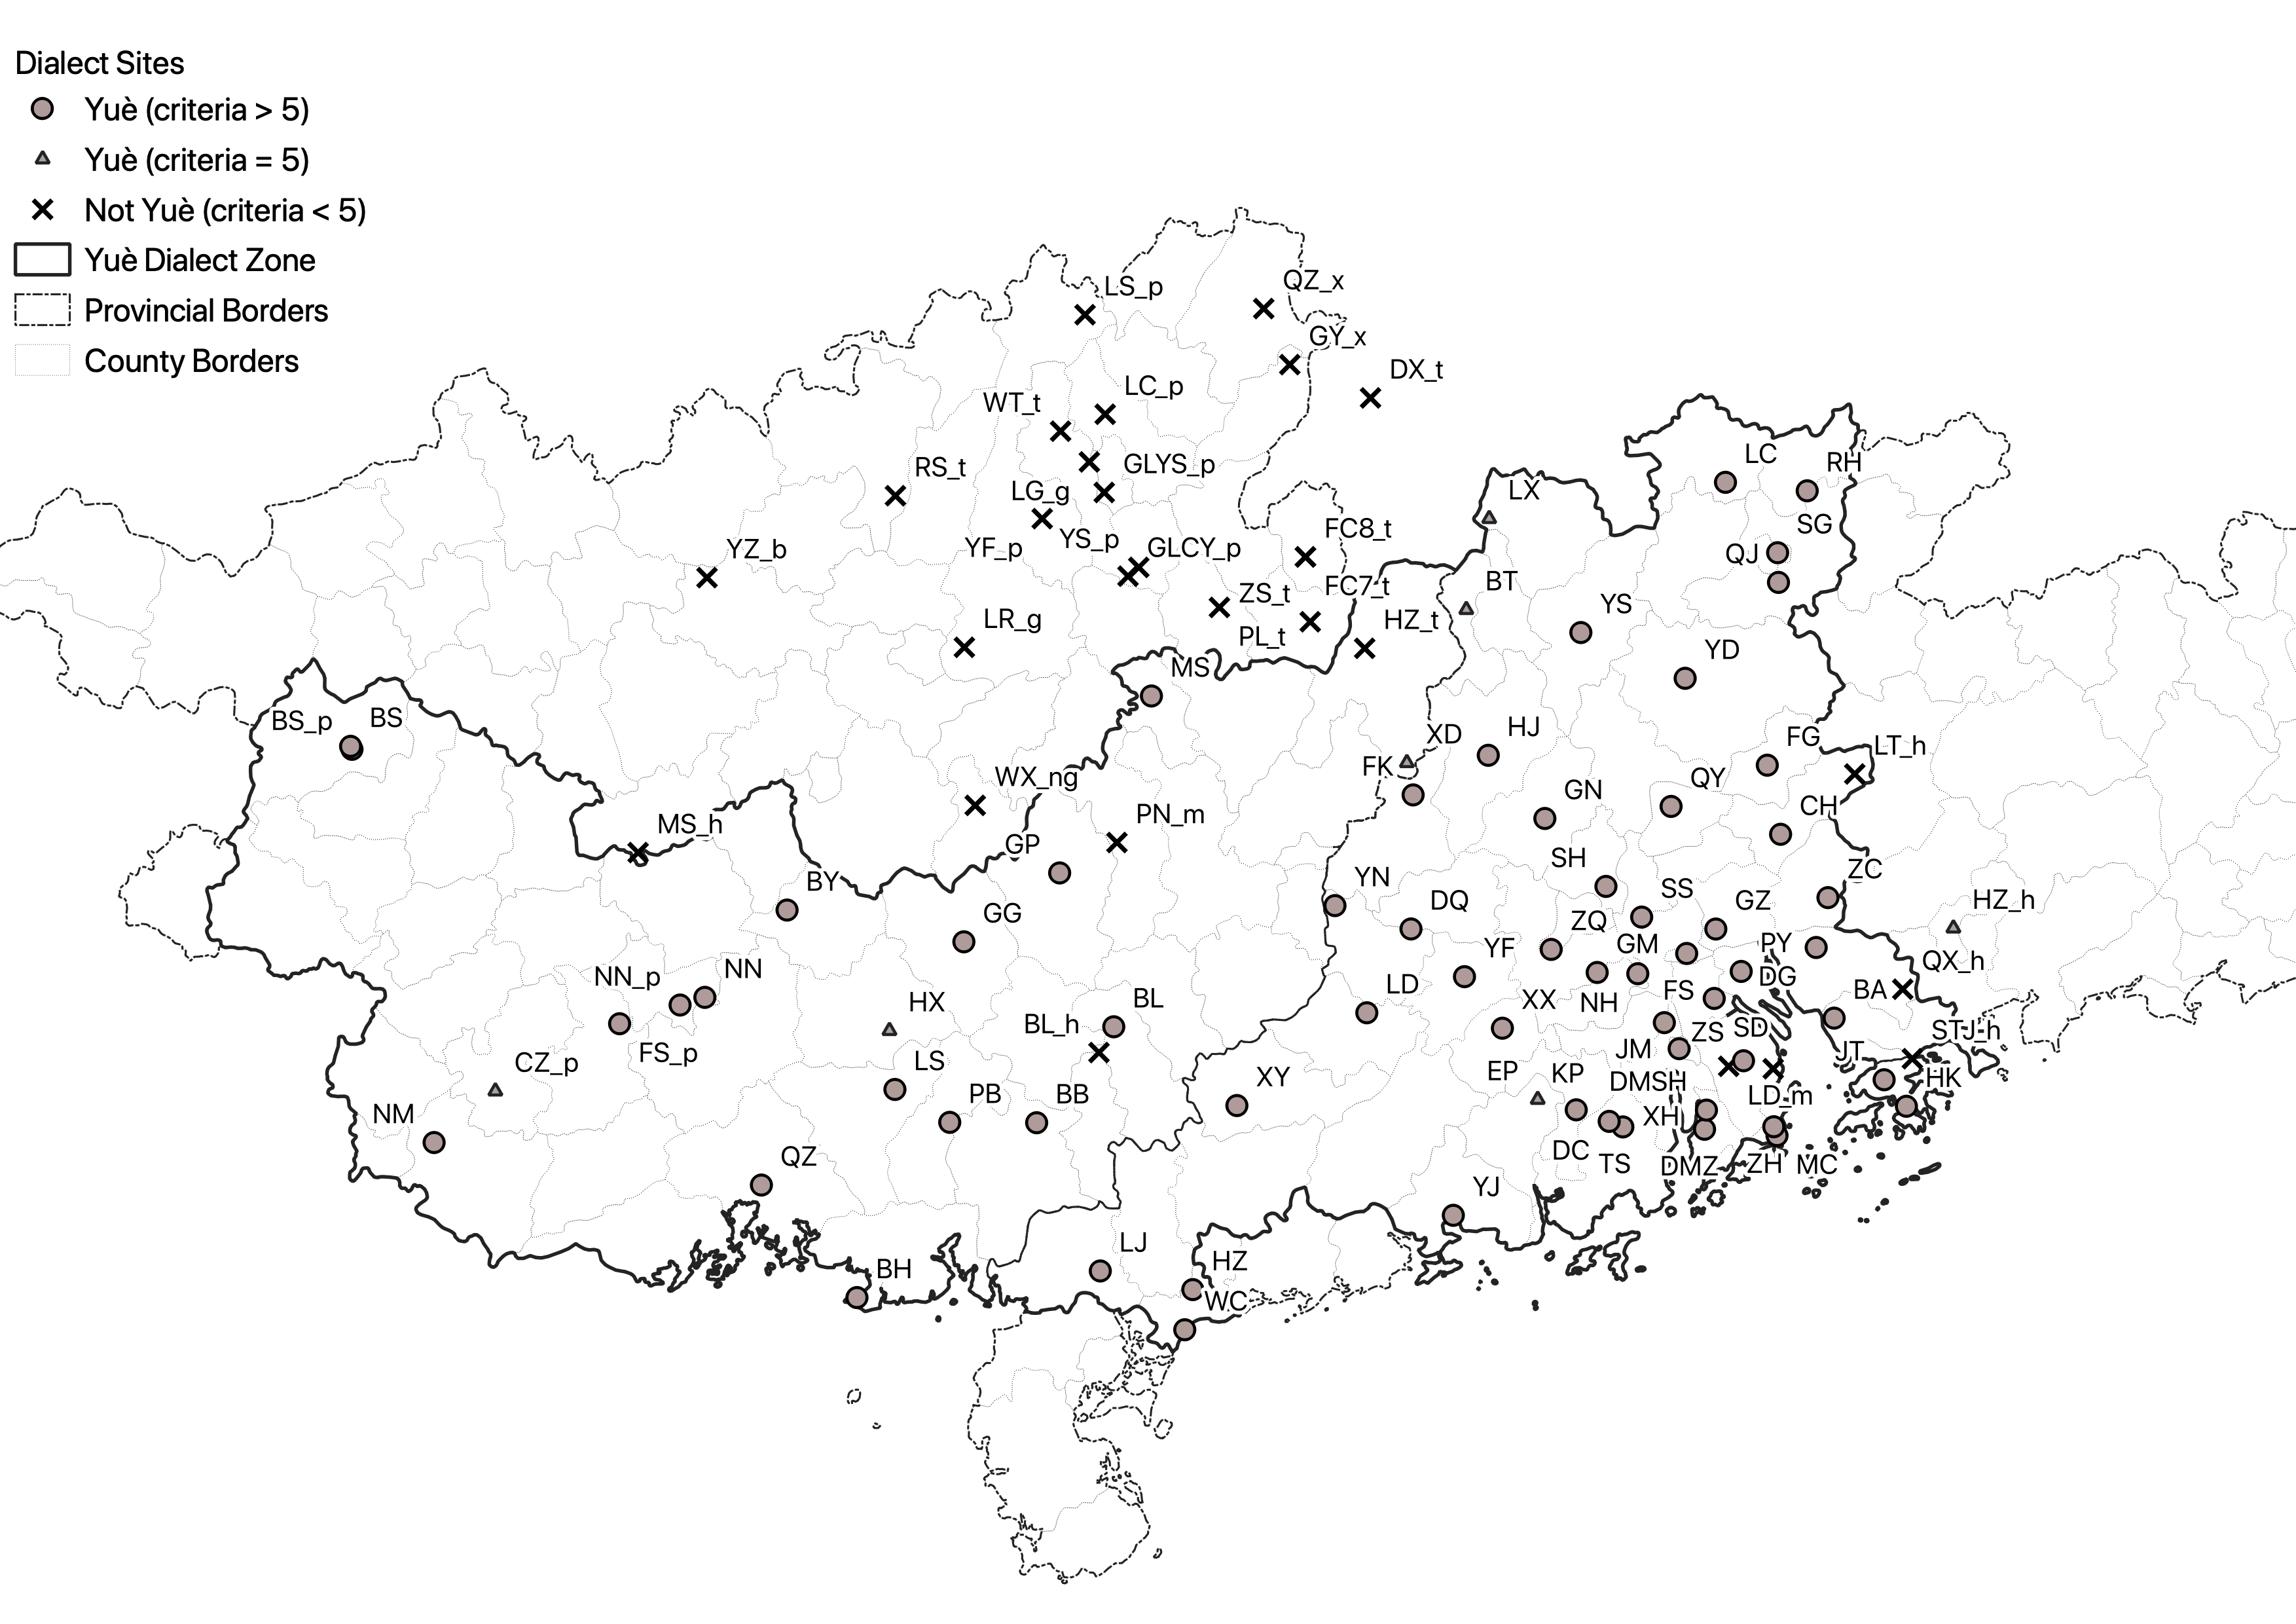
\includegraphics[width=.9\linewidth]{./cy_all_lex.png}
\end{center}
\end{frame}

\section{Introduction to Dialectometry}
\label{sec:orgaa5f3eb}
\begin{frame}[label={sec:org0d33016}]{Dialectometry}
\begin{columns}
\begin{column}{0.5\columnwidth}
\begin{block}{What is it?}
\begin{itemize}
\item The use of computational and quantitative techniques in dialectology
\item Measure the degree of linguistic similarity (or distance) between dialects
\item Relate these measurements to geographic distance and plot them
\end{itemize}
\end{block}
\end{column}
\begin{column}{0.5\columnwidth}
\begin{block}{Why use it?}
\begin{itemize}
\item Visualize migration, contact, and cultural boundaries
\item Obtain a synchronic classification
\item Create high quality maps using GIS
\item Useful for education, language planning, etc.
\end{itemize}
\end{block}
\end{column}
\end{columns}
\end{frame}
\begin{frame}[label={sec:org86fb115}]{The Isogloss Method}
\begin{columns}
\begin{column}{0.5\columnwidth}
\begin{block}{Process}
\begin{itemize}
\item Select linguistic differences
\item Draw lines on map to mark boundaries of differences
\item Seek out bundles of isoglosses
\end{itemize}
\end{block}
\end{column}
\begin{column}{0.5\columnwidth}
\begin{block}{Limitations}
\begin{itemize}
\item Possible bias in selecting differences
\item Can't directly compare non-contiguous regions
\item Laborious
\item Difficult to interpret results
\end{itemize}
\end{block}
\end{column}
\end{columns}
\end{frame}
\begin{frame}[label={sec:org36b434c}]{Yuè Chinese Isoglosses}
\textcite[p. 41]{yue-hashimoto1988preliminaryinvestigation}
\begin{center}
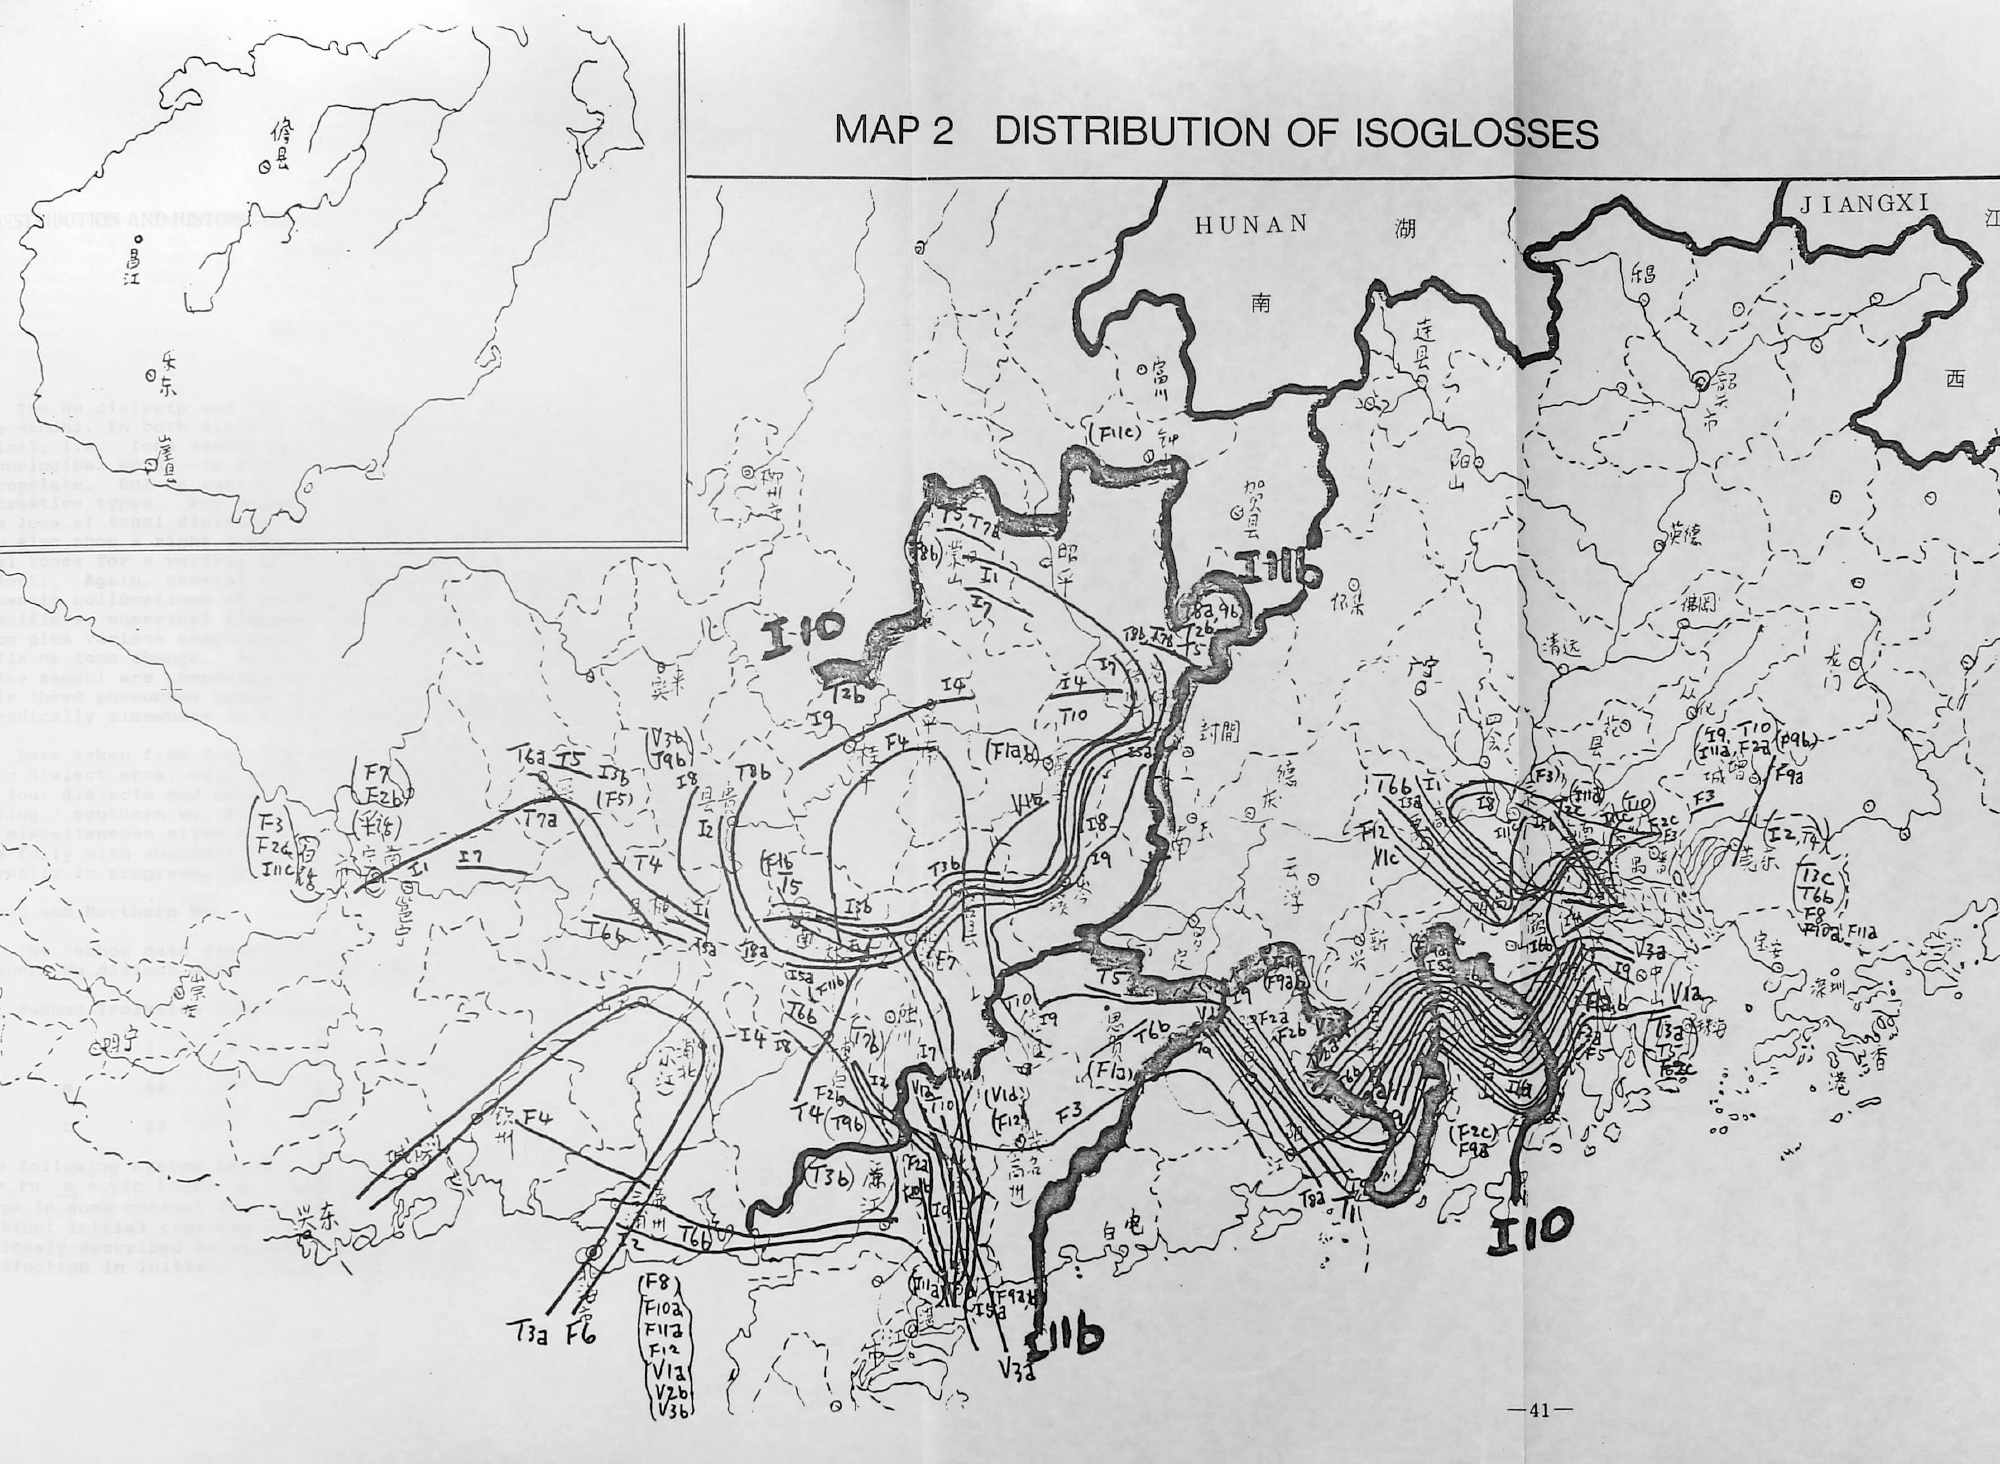
\includegraphics[width=.9\linewidth]{Screen Shot 2022-05-21 at 3.40.46 PM.png}
\end{center}
\end{frame}
\begin{frame}[label={sec:org394d849}]{The Advantages of Dialectometry}
\begin{itemize}
\item Can use data from all linguistic levels
\item Data represents modern dialects directly
\item Includes all data without biased selections
\item Uses data maximally
\item Can compare areas that are not close
\item Clear results
\end{itemize}
\end{frame}
\begin{frame}[label={sec:org595a31a}]{Gabmap}
\textcite{nerbonne2011gabmapaweb}
\begin{itemize}
\item Online Dialectometry Web App
\item Based on earlier RuG/L04 program
\item \url{http://www.let.rug.nl/\~kleiweg/L04/webapp/}
\end{itemize}
\end{frame}
\section{Measuring Lexical Similarity}
\label{sec:orgee41c09}
\begin{frame}[label={sec:orge84d444}]{Categorical Data}
\begin{center}
\begin{tabular}{lllll}
Site & to rain & morning & salt & \ldots{}\\
\hline
GZ & 落雨 & 聽日 & 鹽 & \ldots{}\\
TS & 落水 & 天早 & 上味 & \ldots{}\\
\end{tabular}
\end{center}
\begin{columns}
\begin{column}{0.5\columnwidth}
\begin{block}{Categorical Distance}
\textcite{seguy1971relationentre} \\
For distance between two dialects:
\begin{itemize}
\item same words as 0 (no distance)
\item different words as 1
\item take average for word list
\end{itemize}
\end{block}
\end{column}
\begin{column}{0.5\columnwidth}
\begin{block}{Weighted Difference Value}
\textcite{goebl1984dialektometrischestudien}
\begin{itemize}
\item \emph{gewichteter Identitätswert}
\item weight words by the frequency they appear answer to word list item
\item emphasize less common responses
\end{itemize}
\end{block}
\end{column}
\end{columns}
\end{frame}
\begin{frame}[label={sec:org769d2a7}]{Limitations of Categorical Yuè Data}
\begin{itemize}
\item Orthography not standard across regions or surveys
\item No accepted \emph{zi} for some morphemes
\item Even broad transcriptions not very similar
\item Judging which words are the ``same'' not always trivial
\end{itemize}
\end{frame}
\begin{frame}[label={sec:orgea8c843}]{String Edit (Levenshtein) Distance}
The method comes from \textcite{levenshtein1966binarycodes}. Applied to gauge lexical similarity in \textcite{nerbonne2003lexicaldistance}.
\begin{itemize}
\item Smallest set of operations to transform one string (of segments) to another
\item Insert, delete, substitute
\item Normalize by length of compared strings
\item Follow \textcite{yangcastro2008representingtone} to handle tone
\end{itemize}

GZ to BA
\begin{center}
\begin{tabular}{llllll}
s & i & k & L & E & \\
s & e & ʔ & L & E & \\
\hline
 & 1 & 1 &  &  & 2\\
\end{tabular}
\end{center}
\end{frame}

\begin{frame}[label={sec:org1cb0736}]{Local Incoherence}
\textcite{nerbonnekleiweg2007dialectologicalyardstick} \\
\(I_l = \frac{1}{n}\displaystyle \sum_{i=1}^{n} \frac{D_i^L - D_i^G}{D_i^G}\)
\begin{itemize}
\item Average of the geographic distance between the most linguistically similar site for each site normalized by the distance of the actual closest site
\end{itemize}

\begin{center}
\begin{tabular}{lr}
Method & Local Incoherence\\
\hline
Binary & 1.10\\
Weighted & 0.95\\
Levenshtein & 1.34\\
\end{tabular}
\end{center}
\end{frame}


\section{Linguistic and Geographic Distance}
\label{sec:orgdaf5864}
\begin{frame}[label={sec:org62afada}]{Difference Map}
\begin{center}
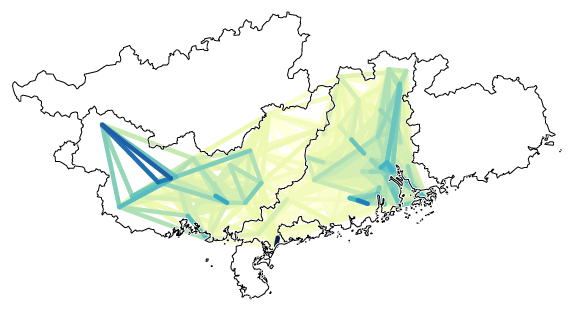
\includegraphics[width=.9\linewidth]{diff.png}
\end{center}
\end{frame}
\begin{frame}[label={sec:org62a31a2}]{Linguistic Difference ↔ Geographic Distance}
\begin{center}
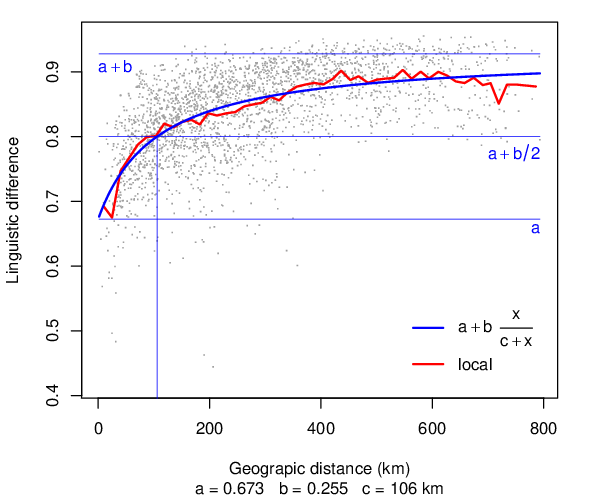
\includegraphics[width=.9\linewidth]{plot01.png}
\end{center}
\end{frame}
\begin{frame}[label={sec:orgb6f69b3}]{Reference Point: Guangzhou}
\begin{center}
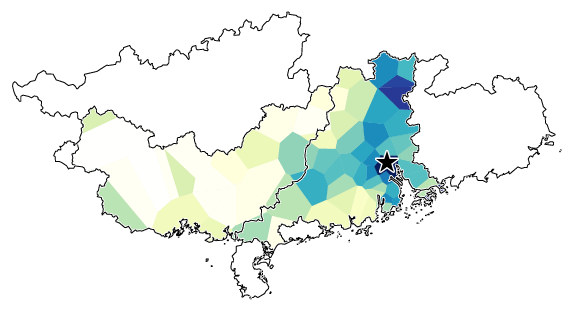
\includegraphics[width=.9\linewidth]{curmap_gz.png}
\end{center}
\end{frame}
\begin{frame}[label={sec:org16e097f}]{Reference Point: Taishan}
\begin{center}
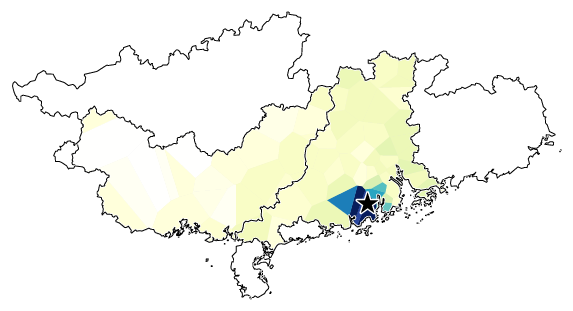
\includegraphics[width=.9\linewidth]{curmap_ts.png}
\end{center}
\end{frame}
\begin{frame}[label={sec:org5c66c81}]{Reference Point: Guangning}
\begin{center}
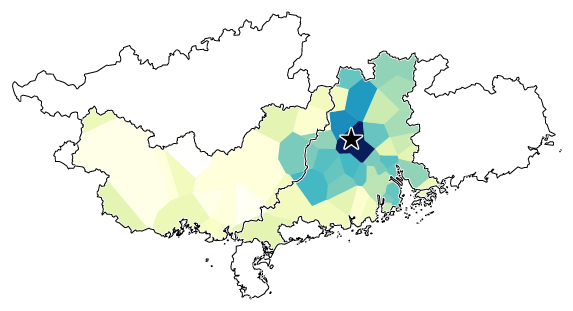
\includegraphics[width=.9\linewidth]{curmap_gn.png}
\end{center}
\end{frame}
\begin{frame}[label={sec:org1057082}]{Reference Point: Nanning (Pinghua)}
\begin{center}
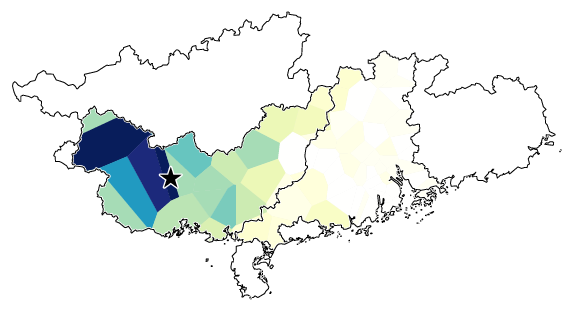
\includegraphics[width=.9\linewidth]{curmap_nn_p.png}
\end{center}
\end{frame}

\section{Multidimensional Scaling}
\label{sec:org974a7f6}
\begin{frame}[label={sec:orgaddf802}]{Multidimensional Scaling}
\textcite{kruskal1964nonmetricmultidimensional}
\begin{itemize}
\item Multidimensional Scaling = MDS
\item Technique to estimate relative positions of points in an arbitrary multidimensional space using relative distances as input
\item Useful for understanding the gradual nature of boundaries, but is a bit of sensory overload
\item Not always precise
\end{itemize}
\end{frame}
\begin{frame}[label={sec:org31ece59}]{In Two Dimensions}
\begin{center}
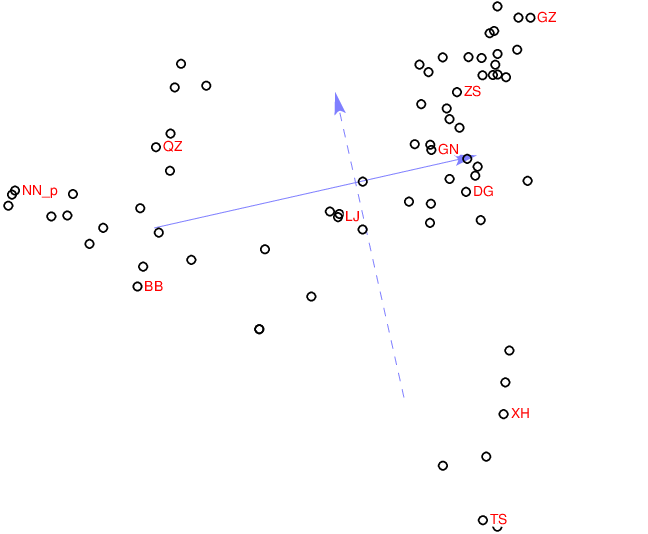
\includegraphics[width=0.75\textwidth]{plot2d.png}
\end{center}
r = 0.76
\end{frame}

\begin{frame}[label={sec:orgc180c21}]{In Three Dimensions}
\begin{center}
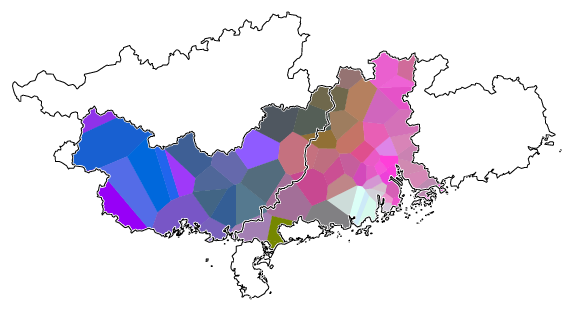
\includegraphics[width=.9\linewidth]{standard.png}
\end{center}
r = 0.81
\end{frame}

\section{Clustering}
\label{sec:orgdb9d449}
\begin{frame}[label={sec:org18d386d}]{Discrete Clustering}
\begin{itemize}
\item Given the distances between sites, cluster sites so that sites in the same cluster are more linguistically similar to each other than to those in other clusters.
\item Prone to produce very different results based on even small fluctuations in the data.
\item[{UPGMA}] Unweighted Pair Group Method using Arithmetic averages \\
cophenetic distances (distances in the clusters) match original distances most closely
\item[{WPGMA}] Weighted Pair Group Method using Arithmetic averages \\
for irregular distribution
\item[{Ward's Method}] Minimum Variance \\
Gives clusters of roughly even size
\end{itemize}
\end{frame}
\begin{frame}[label={sec:orge511255}]{Weighted Average Dendrogram}
\begin{center}
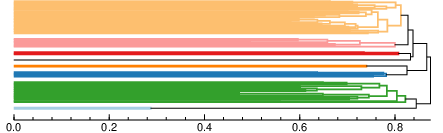
\includegraphics[width=.9\linewidth]{denwa8col.png}
\end{center}
\end{frame}
\begin{frame}[label={sec:org0674f8b}]{Weighted Average Map}
\begin{center}
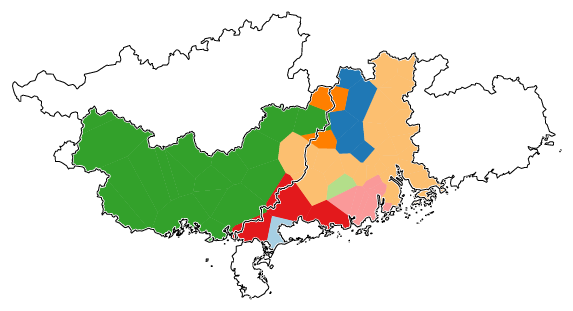
\includegraphics[width=.9\linewidth]{mapwa8col.png}
\end{center}
\end{frame}
\begin{frame}[label={sec:org3a12f0e}]{Cluster Verification}
\begin{center}
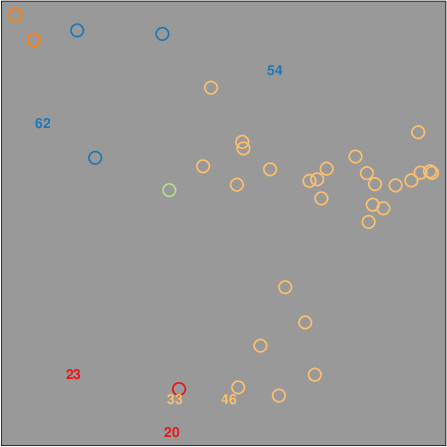
\includegraphics[width=0.6\textwidth]{plot_wa_8_2_3_6_7_8.png}
\end{center}
\end{frame}
\begin{frame}[label={sec:org2591b24}]{Fuzzy Clustering}
\textcite{nerbonne2008projectingdialect}
\begin{itemize}
\item Prevent instability by repeatedly clustering while introducing noise. Clusters that occur the most often are the stablest.
\item Process:
\begin{itemize}
\item Cluster repeatedly (n=100), randomly adding noise to the distance matrix (0 ≤ r ≤ 0.2) each iteration
\item Count how many times certain clusters form in these repeated clusterings to approximate certainty of clustering
\item Combine analysis into composite cluster
\end{itemize}
\item Can project results to geography using cophenetic distances
\end{itemize}
\end{frame}
\begin{frame}[label={sec:org6e2e9fd}]{Probabilistic Dendrogram}
\begin{center}
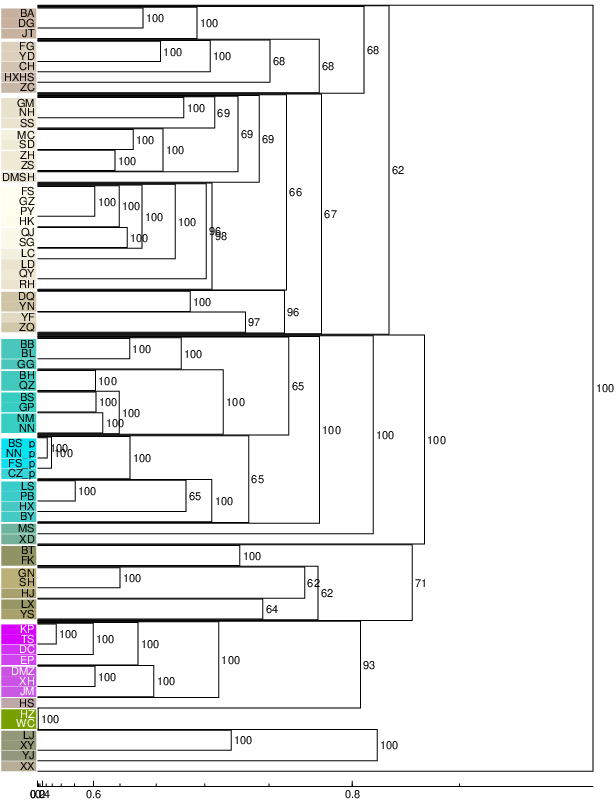
\includegraphics[angle=90,width=.9\linewidth]{prob.png}
\end{center}
\end{frame}
\begin{frame}[label={sec:org60275c4}]{Fuzzy Clustering Map}
\begin{center}
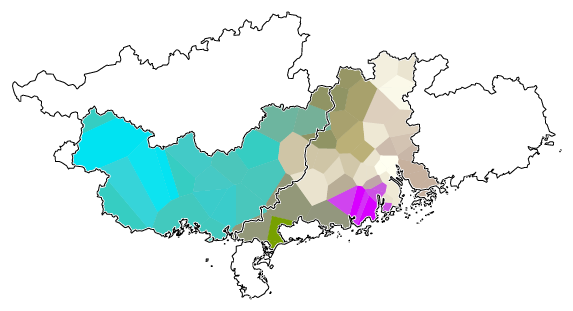
\includegraphics[width=.9\linewidth]{ccc.png}
\end{center}
\end{frame}

\section{Wrap-up}
\label{sec:org732de4c}
\begin{frame}[allowframebreaks,label=]{Bibliography}
\printbibliography[heading=none]
\end{frame}
\begin{frame}[label={sec:org14946a1}]{Questions}
\end{frame}
\begin{frame}[label={sec:org9e136a9}]{Thank you}
\end{frame}
\end{document}